\documentclass[9pt,b5j,papersize]{jsarticle}
\usepackage[dvipdfmx]{graphicx}
\usepackage{wrapfig}
\usepackage{float}
\usepackage{otf}
\usepackage{longtable}
\usepackage{ulem}
\usepackage{ascmac}
\usepackage{titlesec}
\usepackage{multicol}
 \usepackage{url}
%%%脚注を文末に出す
%\usepackage{endnotes}
%\let\footnote=\endnote
%\renewcommand{\theendnote}{\arabic{endnote})}
%\renewcommand{\notesname}{{\small 註}}
%\def\ennotesize{\normalsize}
%\def\notessize{\normalsize}
%\usepackage{etoolbox}
%\patchcmd{\enoteformat}{1.8em}{0pt}{}{}
%%%
\setlength{\textwidth}{150truemm}      % テキスト幅: 160mm
\setlength{\fullwidth}{\textwidth}     % ページ全体の幅
\setlength{\oddsidemargin}{-10truemm}   % 左余白
\setlength{\topmargin}{-10truemm}       % 上余白
\setlength{\textheight}{210truemm}     % テキスト高さ: 297-(30+30)=237mm
\pagestyle{empty}
%%%文字数と行数を指定する
\makeatletter
\def\mojiparline#1{
    \newcounter{mpl}
    \setcounter{mpl}{#1}
    \@tempdima=\linewidth
    \advance\@tempdima by-\value{mpl}zw
    \addtocounter{mpl}{-1}
    \divide\@tempdima by \value{mpl}
    \advance\kanjiskip by\@tempdima
    \advance\parindent by\@tempdima
}
\makeatother
\def\linesparpage#1{
    \baselineskip=\textheight
    \divide\baselineskip by #1
}
%%%見出しの表示方法変更
%\titleformat*{\section}{\large\bfseries\textgt}
%\titleformat*{\subsection}{\normalsize\bfseries\textgt}{\filright(\,\thesubsection\,)}
%%%

\begin{document}
% 1行あたりの文字数指定
\mojiparline{50}
% 1ページあたり行数の指定
\linesparpage{44}
%%%%%%%%%%%%%%%%

\begin{center}
{\LARGE 考古学情報の再現可能性}

\vspace{1\baselineskip}
{\Large 〜バージョン管理システムGitを利用した調査データの管理と公開〜}
\end{center}

\vspace{2\baselineskip}

\begin{flushright} {\large 石 井 淳 平} \end{flushright}

\vspace{1\baselineskip}

\begin{multicols}{2}

%%%%
\noindent
{\large はじめに}

発掘調査記録をオープンデータとして活用するための方策として、GitHubに代表されるバージョン管理+共有サービスの利用事例を報告する。図書として刊行された発掘調査報告書は、情報の固定という面で優れているが、報告書作成に利用された調査記録や中間成果物へのアクセシビリティが低く、再現性が低いことが問題である。このことは、考古学情報の真正性の問題に関わるとともに、考古学情報の社会的利用にも関わる問題である。Gitを使用し、一次情報である現場図面や写真、最終的な報告書に至る中間成果物すべての改変履歴を記録することで考古学情報の真正性と再現可能性が担保される。また、Gitの機能を利用したウェブサービスであるGitHubにより考古学情報の作成に関わった調査記録の公開が実現する。

本報告では、北海道南部の箱館戦争遺跡の調査におけるGitによるバージョン管理とGitHubを利用したデータ共有の実践例を紹介し、手法やノウハウを報告する。

%%%%
\noindent
{\large 1.ブラックボックス化する考古学情報}

考古学情報の保存・公開に用いられる媒体については、紙でもPDFでも情報の再現可能性としては同質である。考古学情報における紙媒体(あるいはPDF)について文化庁は「刊行後の改変が困難であるため,情報の真正性が確保できる」(文化庁2017,p12)としているが、「真正性」の定義が筆者と異なっており、必ずしも肯定できない。筆者は考古学情報作成に関わる一次情報や中間成果物を再利用可能なデータ群として流通させることが考古学情報の「真正性」確保と考古学情報の社会的利用のために必要と考えている。

例えば、遺物の整理分類に使用された「遺物台帳」を元に作成された遺物集計表が報告書に掲載されているとする。しかし、最終的な報告書しか手にすることができない者にはこれらの集計作業が適切に行われたかどうかを判断するすべはない。そのような考古学情報の「真正性」を評価することはできない、というのが筆者の考え方だ。

%%%%
\noindent
{\large 2.考古学情報の「真正性」}

考古学情報の再現可能性を高めることは、考古学情報の「真正性」を高めることにほかならない。考古学情報の「真正性」を文化財における「真正性(authenticity)」に引きつけて表現すると次のようになろう。

\begin{itemize}
\item 考古学情報の価値は真正性によって評価される
\item そのためには考古学情報の作成に使用された情報源が信頼できる度合いが評価されなければならない
\item どのようなプロセスで考古学情報が作成されたのかに関する情報が真正性の評価には必須である
\end{itemize}

つまり考古学情報作成プロセスを明示することが、考古学情報の真正性を評価するための第一歩となる。どのような調査記録が選択され、どのような処理を経て最終的な考古学情報として成立したのかに関する情報が真正性を評価する基本となる。

%%%%
\noindent
{\large 3.Gitを利用した発掘調査記録管理}

以上のような調査記録管理の手法としてGitを用いたバージョン管理とGitHubによるデータ共有を提案する。Gitの使用によって、「どのような改変が」、「いつ」、「誰によって」行われたのかが明示的になる。GitHubのようなデータ共有環境を利用することで、変更履歴が明確なデータ群を誰でも再利用できる。

Gitの主な機能は情報の変更単位ごとに履歴を作成することである。Gitによる変更履歴の登録によって「いつ、どのような変更が、誰によって行われたのか」が明確になる。その結果、最終成果物からは知ることができない考古学情報編集作業の工程と使用されたデータがGitの履歴に残される。Gitには消去、改変された過去の記録も潜在的に保存されているため、考古学情報作成にかかわる全ての記録が保存されることとなる。

%%%%
\noindent
{\large 4.Git利用の実際}

Gitはコマンドラインで操作されることが多く、筆者も基本的にはコマンドラインで操作している。
ただし、Gitには秀逸なGUIクライアントソフトが数多く開発されており(GitKraken、GitCola、SourceTreeなど)、これらのソフトウェアによりGitを直感的に操作することが可能である。GUIクライアントソフトの利用によりコマンド入力から解放され、変更履歴や変更内容が視覚的に一覧できるメリットがある。

Gitでの基本的な作業は「commit」と呼ばれる変更履歴の登録である。特定のディレクトリ(例えば発掘調査報告書作成用のディレクトリ)に対して行われた変更の全てがGitのリポジトリ(データベースのようなもの)に登録される。登録の際に適切なコメント(たとえば「土坑1の断面図を修正」など)を付すことで変更内容が第三者にもわかるようになる。

%%%%
\noindent
{\large 5.北海道北斗市二股台場調査でのGit利用}

筆者らが取り組んでいる北海道北斗市二股台場の測量調査(野村ほか2017)では、GitHubによる調査記録の公開(\url{ https://github.com/IshiiJunpei/Futamata})を行っている。

\begin{figure}[H]
\centering
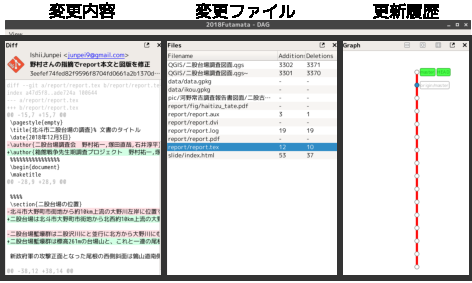
\includegraphics[width=1\columnwidth]{fig/01.pdf}
\caption{二股台場調査のGit情報(GitColaによるGUI表示)}
\label{hutamata}
\end{figure}

調査関係者が日常的に顔をあわせて作業する環境にないため、調査情報をリモートで共有する必要があったこと、複数の調査者が調査記録の編集に関わることから、作業重複を避ける工夫が必要となった。そのため、GitHubを利用し、調査記録更新にかかる公正性の確保と作業重複の回避を行った。

図\ref{hutamata}は二股台場調査記録にかかるGitのログである。右ペインはGitの更新履歴を示す。中央ペインは変更が行われたファイルの一覧である。変更が行われたファイルを選択すると左ペインにファイルの内容と変更箇所が示される。ここでは共同調査者からの指摘で報告文本文の修正と図版データの修正を行った内容が表示されている。このように全ての変更履歴が変更後の差分とあわせて確認できることがGitを利用する大きなメリットである。

%%%%
\noindent
{\large 6.オープンデータとしての考古学情報}

考古学情報が適切なデータを使用して作成されているか、適切な手順を踏んで作成されているかを判断するためには、調査記録や中間成果物にアクセスできる環境が必要となる。考古学情報の真正性は「情報の固定化」ではなく、すべてのデータにアクセスできる環境の構築によって担保される、というのが筆者の考えだ。

また、オープンソースのソフトウェアのソースコードから必要な部分を切り取って自由に利用できるようになったことで、コンピュータソフトウェアの開発が大きく進んだのと同じように、考古学情報に関わる調査記録や中間成果物を自由に利用できる学問上のメリットははかりしれない。

全国遺跡報告総覧への報告書アップロードも十分とは言えない現状を考えると、筆者のアイディアは時期尚早といえるかもしれないが、考古学情報の保存と公開は、中間成果物を含む全ての情報を対象とし、適切な公開手法と組み合わせて検討していく必要がある。

%%%
\vspace{1\baselineskip}
\noindent
引用参考文献\\
野村祐一,塚田直哉,石井淳平 2017「北斗市二股台場の調査」『第39回南北海道考古学情報交換会』報告資料\\
文化庁 2017『埋蔵文化財保護行政におけるデジタル技術の導入について2』(報告)\\

\end{multicols}

\end{document}
